\subsection{Results}

In this study, participants had an average of 3.0 target sites enabled. They visited at least one target site 67\% of days on average. On each of those days, participants experienced interventions an average of 3.6 times. We did not receive any feedback indicating that participants were aware of patterns in how HabitLab was rotating interventions.

% summary_stats_study1.py
% num domains per user: mean 3.0 stddev 1.8
% fraction time seen: mean 0.96 stddev 0.6
% num sessions per day: mean 3.6 stddev 5.3

% \msb{Report a general statical overview here first. For example, what is the average number of sessions per participants per site per day?}

% Our analysis focuses on two levels of measurement: sessions and days.

% Time on Facebook per day is measured as the total time the user was actively using Facebook in the browser (with "active" being the same definition that the Chrome browser uses - tab focused, window focused, and mouse or keyboard movement within the past minute). The day starts from midnight in the local timezone. Because we excluded users who had HabitLab installed on multiple devices, we are considering only Facebook usage on a single device.

% Time on Facebook per visit is measured as the total time the user was actively using Facebook in a browser tab, from when they visited Facebook until they closed the tab. If the user switches tabs to a different site, the time spent on the other site is not counted towards the current Facebook session time.

% We discarded days on which Facebook was not visited at all. For measurements of time on Facebook per day, we discarded the first day, as the user may install midway through the day so the measured time that day would be an underestimate. For measurements of time on Facebook per day, we discarded any days on which a user attritioned (which can result from uninstalling or disabling the extension), as this would again cause the measured time to be an underestimate of the actual time spent on site that day.

% We analyzed our data using a linear mixed model. We used this because we have multiple samples from each user, but the number of samples from each user and in each condition is variable (because users may attrition before they completed all conditions, they may not visit a site on a particular day), which violates the assumptions of the repeated-measures ANOVA.

% how to report data from a linear mixed model: https://arxiv.org/ftp/arxiv/papers/1308/1308.5499.pdf

% You	would	report	this result	the	following	way:
% “…	 politeness	 affected	 pitch	 (χ2(1)=11.62,	 p=0.00065),	 lowering	 it	 by	
% about	19.7 Hz	± 5.6	(standard	errors)	…”
\subsubsection{Effectiveness of interventions over time}
First we examine whether interventions decrease in effectiveness over time within the static condition. If so, rotation may be a viable strategy.



%Interventions decrease in effectiveness over time (as evidenced by longer visit times on site), both if we measure it according to the number of days on which the intervention has been previously seen at least once, or if we measure it according to number of total times that the intervention has been seen.

The likelihood ratio test confirms that the number of days the user had seen the static intervention affected the log of time spent on a domain per day ($\chi^{2}(1) = 4.69, p < 0.05$), supporting H\ref*{hyp:decreaseovertime}. Each day the intervention has been previously seen increased the log time spent by 0.225 (Table~\ref{tab:effectiveness_sessions_alldomain_vs_num_days_same}). By exponentiating the log estimates, this translates into an increase of 25\% on top of a baseline 117 seconds per day for each additional day the user were exposed to the static intervention. %during the study. %Note that since the dependent variable is log time rather than raw time, this 15\% estimated increase is multiplicative for each additional day. 
%An alternative method of analysis, where we measure the raw number of times the intervention has been seen instead of the number of days it has been seen, yields the same results. \msb{still correct?} %\msb{does an equivalent analysis at the day level yield the same results? otherwise why did we make such a big deal of having both session and day data? If we're going to report both, we need to report both for all studies. Otherwise we need to cut and use just one.} %Restricting analysis to just Facebook also yields the same results.

%\msb{This paragraph doesn't make sense to me: the method section said that this dataset considered only static days:} Note that we observed a significant decline in effectiveness if we analyze days where users were assigned to the static condition, but the decline is not significant on days when the user is in the rotation condition. This suggests that if interventions decline in effectiveness in the rotation condition, it is occurring at a rate too slow to be observed with our study.

% Table created by stargazer v.5.2 by Marek Hlavac, Harvard University. E-mail: hlavac at fas.harvard.edu
% Date and time: Wed, Apr 18, 2018 - 18:19:53
% Table created by stargazer v.5.2 by Marek Hlavac, Harvard University. E-mail: hlavac at fas.harvard.edu
% Date and time: Wed, Apr 18, 2018 - 18:50:23
\begin{table}[tb] \centering 
  \caption{Within the static condition, interventions decline in effectiveness. Longer visit lengths increase with the number of days seeing the same static intervention.} 
  \label{tab:effectiveness_sessions_alldomain_vs_num_days_same} 
\begin{tabular}{@{\extracolsep{5pt}}lc} 
\\[-1.8ex]\hline 
\hline \\[-1.8ex] 
 & \multicolumn{1}{c}{\textit{Dependent variable:}} \\ 
\cline{2-2} 
\\[-1.8ex] & Log time spent per day \\ 
\hline \\[-1.8ex] 
 Number of days the user had seen the static intervention & 0.225$^{*}$ \\ 
  & (0.097) \\ 
  (Intercept) & 4.759$^{***}$ \\ 
  & (0.392) \\ 
 \hline \\[-1.8ex] 
Observations & 124 \\ 
\hline 
\hline \\[-1.8ex] 
\textit{Note:}  & \multicolumn{1}{r}{$^{*}$p$<$0.05; $^{**}$p$<$0.01; $^{***}$p$<$0.001} \\ 
\end{tabular}
\vspace{1em}
\end{table} 


%First we ran a Shapiro test of normality to find that the response variable (log of session times) is indeed normally distributed: W = 0.97751, p-value = 3.724e-06 TODO it looks like it's not actually, probably need to switch to a GLMM

%shapiro.test(data_facebook$log_time_spent)



%We used a chi-squared test to compare the following two linear mixed effects models for predicting the log of time spent on Facebook per session:

%Full model: number of days the intervention has been previously seen [fixed effect], intervention [fixed effect], user [random effect]

%Reduced model: intervention [fixed effect], user [random effect]

% results <- lmer(log_time_spent ~ num_days_intervention_seen_at_least_once + as.factor(intervention) + (1|install_id), data = data_facebook)
% resultsnull <- lmer(log_time_spent ~ as.factor(intervention) + (1|install_id), data = data_facebook)

%The number of days the intervention has been previously seen affected the log of time spent on Facebook per visit ($\chi^{2}(1)$ = 4.4276, p = 0.03536), with each day the intervention has been previously seen increasing it by an estimate of 0.06738 (standard error = 0.03171, t-value = 2.125) from an intercept of 3.82230 (standard error = 0.29295, t-value = 13.047).

%            Df    AIC    BIC  logLik deviance  Chisq Chi Df Pr(>Chisq)  
%resultsnull  7 1622.2 1650.6 -804.10   1608.2                           
%results      8 1619.8 1652.2 -801.88   1603.8 4.4276      1    0.03536 *

%                                                    Estimate Std. Error t value
%(Intercept)                                          3.82230    0.29295  13.047
%num_days_intervention_seen_at_least_once             0.06738    0.03171   2.125

%This translates into an increase of 7\%, or 3 seconds per visit each additional day that an intervention has been previously seen (we calculated these using $firstday=e^{intercept}=e^{3.82230}=46$ and $nextday=e^{intercept+estimate}=e^{3.82230+0.06738}=49$ -- note that since the linear mixed effects model is fitting its estimate to the log of time spent, this estimated increase is multiplicative when translated back to raw time).

%QUESTION: do we want to include the below at all? \msb{no, I compressed it}

%We used a chi-squared test to compare the following two linear mixed models for predicting the log of time spent on Facebook per session:

%Full model: number of times the intervention has been previously seen [fixed effect], intervention [fixed effect], is it the first time the user is visiting Facebook today [fixed effect], user [random effect]

%Reduced model: intervention [fixed effect], is it the first time the user is visiting Facebook today [fixed effect], user [random effect]

%results <- lmer(log_time_spent ~ impression_idx + is_first_visit_of_day + as.factor(intervention) + (1|install_id), data = data_facebook)
%resultsnull <- lmer(log_time_spent ~ is_first_visit_of_day + as.factor(intervention) + (1|install_id), data = data_facebook)

%The number of times the intervention has been previously seen affected the log of time spent on Facebook per visit ($\chi^{2}(1)$ = 4.7703, p = 0.02896), with each time the intervention has been seen increasing it by an estimate of 0.008059 (standard error = 0.003675, t-value = 2.193) from an intercept of 3.283771 (standard error = 0.340267, t-value = 9.651).

%This translates into an increase of TODO 7\%, or 3 seconds per visit each additional time that an intervention has been previously seen (we calculated these using $firsttime=e^{intercept}=e^{3.283771}=46$ and $nexttime=e^{intercept+estimate}=e^{3.82230+0.06738}=49$ -- note that since the linear mixed model is fitting its estimate to the log of time spent, this estimated increase is multiplicative when translated back to raw time).

%                                                     Estimate Std. Error t value
%(Intercept)                                          3.283771   0.340267   9.651
%impression_idx                                       0.008059   0.003675   2.193
%is_first_visit_of_day                                0.676552   0.214924   3.148

%            Df    AIC    BIC  logLik deviance  Chisq Chi Df Pr(>Chisq)  
%resultsnull  8 1617.4 1649.8 -800.72   1601.4                           
%results      9 1614.7 1651.1 -798.33   1596.7 4.7703      1    0.02896 *

\subsubsection{Effectiveness of rotation and static intervention strategies}

%The likelihood ratio test found a significance difference between the full and reduced models predicting effectiveness ($\chi^{2}(1) = 6.31, p < 0.05$), indicating that condition significantly impacted effectiveness. Relative to the rotation condition, static interventions increased the log time spent on Facebook per day by 0.7549 (Table~\msb{REGRESSION TABLE TODO}). Exponentiating for descriptive purposes, this translates into a shift from an estimated 219 seconds per day in the random condition to 466 seconds per day in the rotation condition, an increase of 247 seconds per day.

Next, we compare whether the daily time spent on domains differs between days when participants were in the rotation and static conditions.

The likelihood ratio test found a significance difference between the full and reduced models predicting effectiveness ($\chi^{2}(1) = 4.88, p < 0.01$), indicating that condition significantly impacted effectiveness. Relative to the static condition, rotating interventions decreased the log time spent on domains per day by 0.417 (Table~\ref{tab:effectiveness_same_vs_random}), supporting H\ref*{hyp:rotation}. Exponentiating the coefficients for descriptive purposes, this translates into a shift from an estimated 146 seconds per day in the static condition to 96 seconds per day in the rotation condition, a decrease of 50 seconds (34\%) per day.

%An alternative analysis that yields the same result by looking at time spent per session rather than day is shown in the appendix.

%An alternative analysis that yields the same result is to restrict analysis to Facebook on days where more than 1 intervention was seen.

%The likelihood ratio test found a significance difference between the full and reduced models predicting effectiveness ($\chi^{2}(1) = 9.74, p < 0.005$), indicating that condition significantly impacted effectiveness. Relative to the rotation condition, static interventions increased the log time spent on Facebook per day by 0.7549 (Table~\ref{tab:effectiveness_facebook_same_vs_random}). Exponentiating for descriptive purposes, this translates into a shift from an estimated 212 seconds per day in the random condition to 486 seconds per day in the rotation condition, an increase of 274 seconds per day.

% Table created by stargazer v.5.2 by Marek Hlavac, Harvard University. E-mail: hlavac at fas.harvard.edu
% Date and time: Wed, Apr 18, 2018 - 18:27:32
\begin{table}[tb] \centering 
  \caption{Daily time spent on sites in the static and rotation conditions. Users spend less time per day on sites in the rotation condition.} 
  \label{tab:effectiveness_same_vs_random} 
\begin{tabular}{@{\extracolsep{5pt}}lc} 
\\[-1.8ex]\hline 
\hline \\[-1.8ex] 
 & \multicolumn{1}{c}{\textit{Dependent variable:}} \\ 
\cline{2-2} 
\\[-1.8ex] & Log time spent per day \\ 
\hline \\[-1.8ex] 
 Rotation (baseline: static) & $-$0.417$^{*}$ \\ 
  & (0.190) \\ 
  Block length & 0.018 \\ 
  & (0.048) \\ 
  (Intercept) & 4.981$^{***}$ \\ 
  & (0.346) \\ 
 \hline \\[-1.8ex] 
Observations & 370 \\ 
\hline 
\hline \\[-1.8ex] 
\textit{Note:}  & \multicolumn{1}{r}{$^{*}$p$<$0.05; $^{**}$p$<$0.01; $^{***}$p$<$0.001} \\ 
\end{tabular} 
\vspace{1em}
\end{table} 


%In the days where users were shown the high-novelty condition (where users are shown random interventions each visit), overall time spent on Facebook is less than in the low-novelty days (where users are shown the same intervention).

%First we ran a Shapiro test of normality to find that the response variable (log of daily time spent on Facebook) is indeed normally distributed: W = 0.97878, p-value = 0.118

%shapiro.test(datadays_facebook$log_time_spent)

%We used a chi-squared test to compare the following two linear mixed models for predicting the log of time spent on Facebook per day:

%Full model: condition ("same" or "random") [fixed effect], user [random effect]

%Reduced model: user [random effect]

% results <- lmer(log_time_spent ~ as.factor(condition) + (1|install_id), data = datadays_facebook_withoutattritionday)
% resultsnull <- lmer(log_time_spent ~ (1|install_id), data = datadays_facebook_withoutattritionday)

%The condition affected the log of time spent on Facebook per day ($\chi^{2}(1)$ = 6.3094, p = 0.01201), with condition=same increasing it by an estimate of 0.7549 (standard error 0.2982, t-value = 2.532) from an intercept of 5.3903.

%This translates into an increase of 247 seconds per day (from 219 seconds with random, to 466 in the same condition -- we calculated these using $random=e^{intercept}=e^{5.3903}=219$ and $same=e^{intercept+estimate}=e^{5.3903+0.7549}=466)$.

% you might ask whether this result is significant for sessions too. unfortunately not.

\subsubsection{Attrition due to rotation and static intervention strategies}

\begin{figure}
\centering
	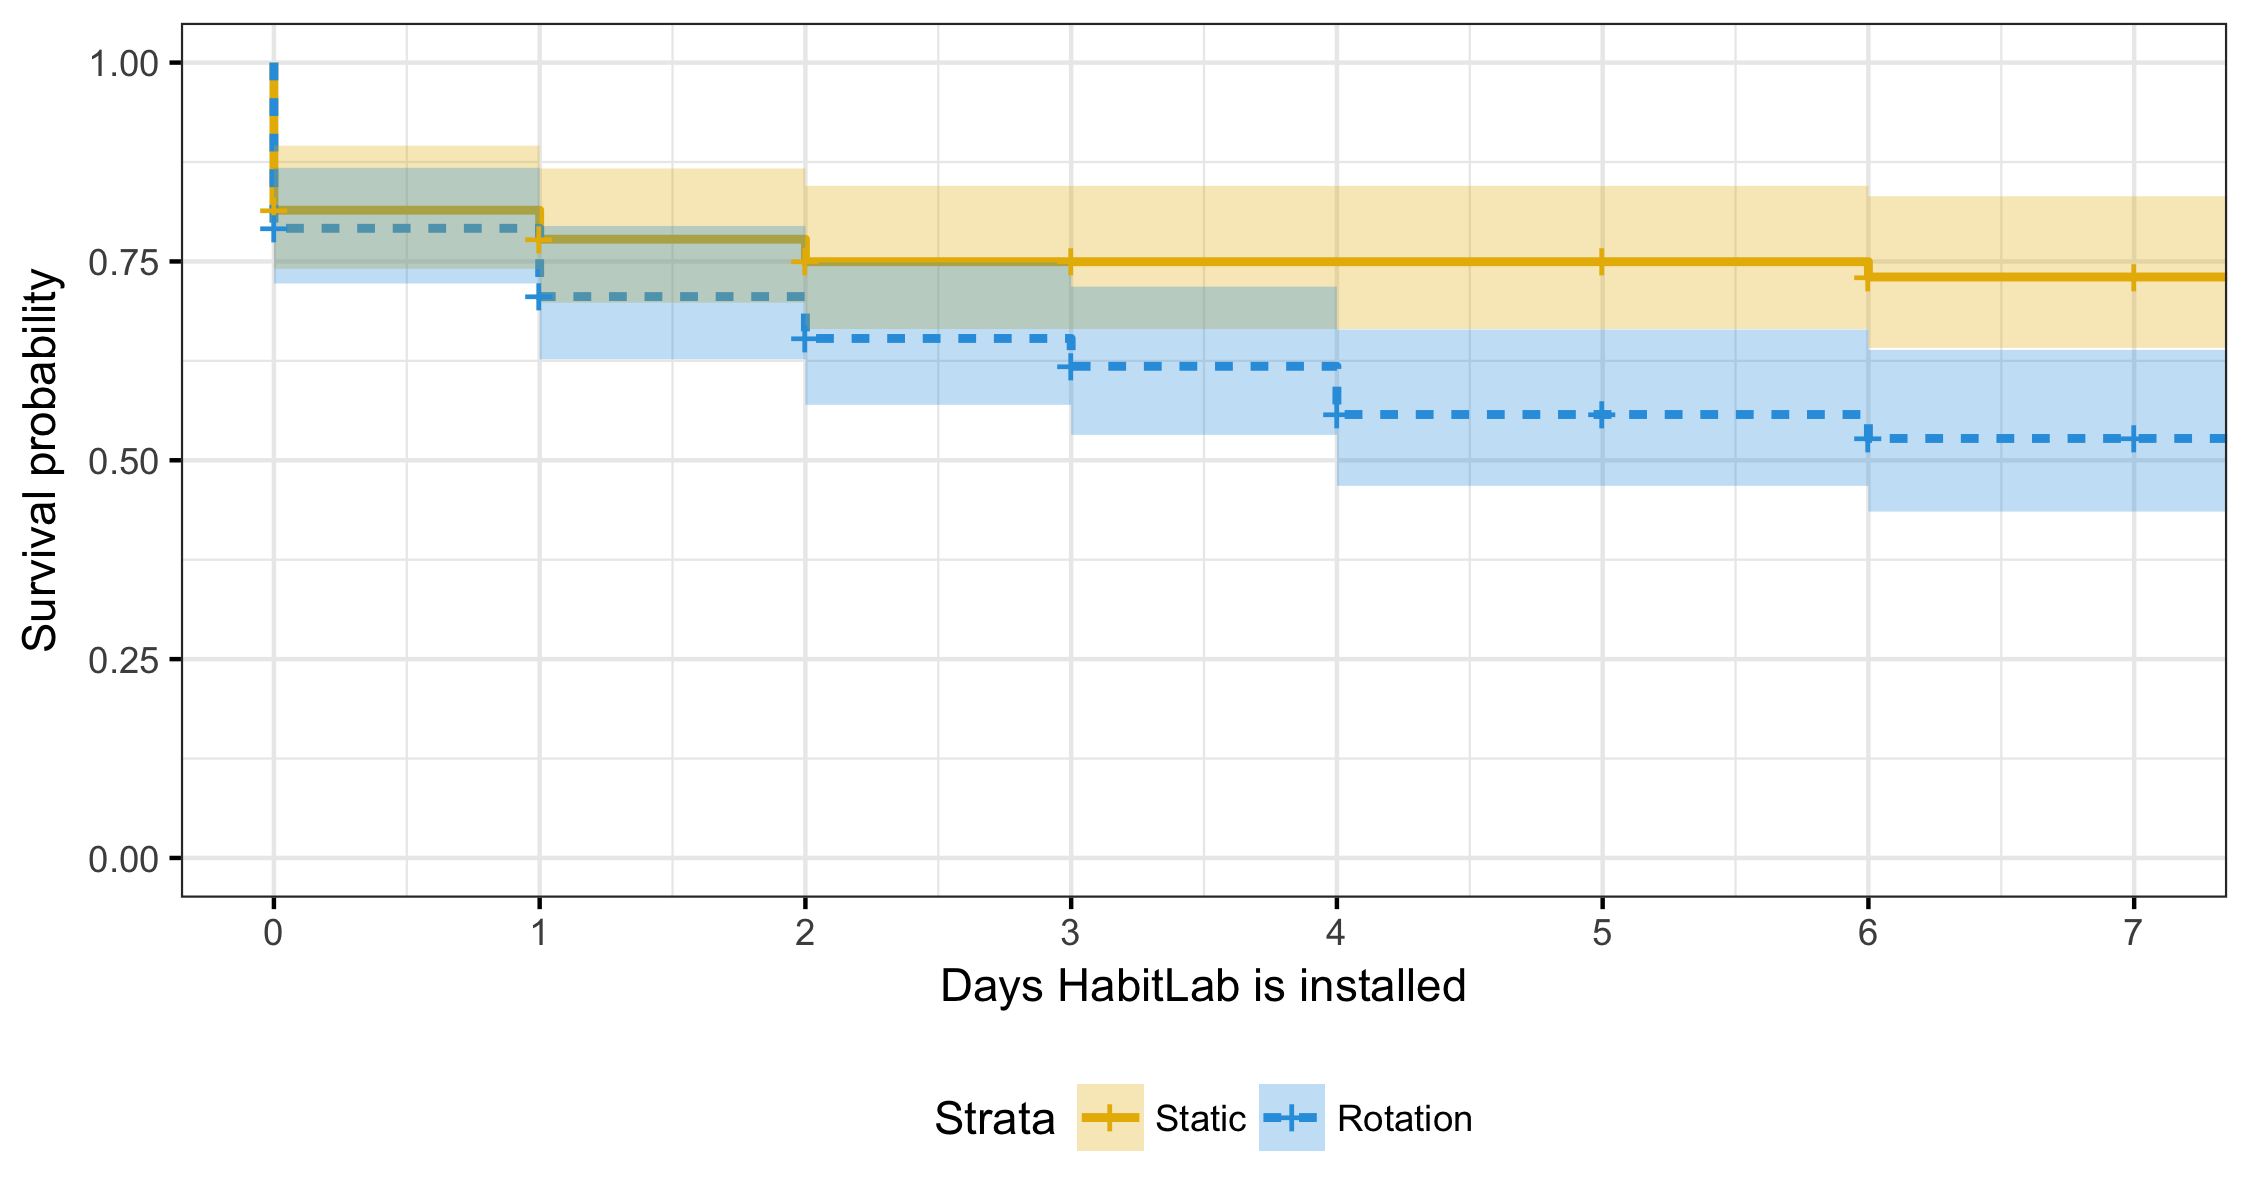
\includegraphics[width=1.0\textwidth]{figures/attrition_within_subjects.png}
	\caption{Rotating interventions increases attrition among users.}
\label{fig:attrition_within_subjects}
\end{figure}

% Table created by stargazer v.5.2 by Marek Hlavac, Harvard University. E-mail: hlavac at fas.harvard.edu
% Date and time: Thu, Apr 19, 2018 - 09:04:52
\begin{table}[tb] \centering 
  \caption{A Cox proportional hazards analysis suggests that the rotation condition substantially increases the hazard of attrition. Coefficients are log hazard ratio, so positive values indicate increased hazard and negative values indicate decreased hazard.} 
  \label{tab:cox_regression} 
\begin{tabular}{@{\extracolsep{5pt}}lc} 
\\[-1.8ex]\hline 
\hline \\[-1.8ex] 
 & \multicolumn{1}{c}{\textit{Dependent variable:}} \\ 
\cline{2-2} 
\\[-1.8ex] & Log hazard ratio \\ 
\hline \\[-1.8ex] 
 Rotation (baseline: static) & 0.544$^{*}$ \\ 
  & (0.249) \\ 
 \hline \\[-1.8ex] 
Observations & 217 \\ 
\hline 
\hline \\[-1.8ex] 
\textit{Note:}  & \multicolumn{1}{r}{$^{*}$p$<$0.05; $^{**}$p$<$0.01; $^{***}$p$<$0.001} \\ 
\end{tabular} 
\end{table} 

% (this is from the within-subjects study)

The Cox proportional hazard regression model comparing the static and rotation conditions found that attrition rates are significantly higher with the rotation condition (Figure~\ref{fig:attrition_within_subjects}, Table~\ref{tab:cox_regression}). After 2 days, 78\% of users remain in the static condition, while only 71\% remain in the rotation condition. After 7 days -- the duration of the longest experiment block -- 68\% of users remain in the static condition, while only 39\% of users remain in the rotation condition. These results support H\ref*{hyp:attrition}.

We considered the possibility that switching between static and rotated interventions contributes to attrition beyond simply rotating them. We analyzed this by comparing the probability of attrition on days where the condition remains the same as the previous day, to days where the condition changes -- either from static to rotated, or from rotated to static. The baseline daily attrition rate is 18\% when staying within the same experimental condition -- 14\% when staying within the static condition, and 20\% when staying within the rotation condition. On the first day after switching from static interventions to rotated interventions, the attrition rate is 36\% -- a significant increase compared to remaining within the same condition (Fisher's exact test, $p < 0.001$). However, switching from rotated interventions to static interventions does not increase the attrition rate -- it remains at 18\%. So we believe these effects are not due to the changes between conditions, but due to the conditions themselves --- switching from static to rotated is experiencing the first instance of a rotation, and it is not surprising that the effect may be larger with the first change.

% (Fisher's exact test, p=0.0006)

%\subsection{Limitations}

%\geza{A limitation of Study 1 is that we cannot conclude with certainty where the cause of the increased effectiveness is from. Is it caused by benefits from the rotation itself? Or might it a side effect of selective attrition -- perhaps users for whom interventions are less effective, happen to be more susceptible to attrition if we are rotating intervention?}

%\geza{An additional limitation is that due to the short durations of our experimental blocks -- with the longest continual condition lasting only 7 days -- we could not observe long-term trends with respect to attrition and effectiveness.}

%TODO change these results to say that attrition is higher when showing random interventions

%There is no significant difference in rates of attrition between days on which users are shown random interventions vs always seeing the same one.

%Because attrition is a binary response variable rather than a normal distribution, we use a Generalized Linear Mixed Model with a binomial family for this analysis.

%We used a chi-squared test to compare the following two generalized linear mixed models for predicting whether or not the user attritions that day:

%Full model: condition ("same" or "random") [fixed effect], user [random effect]

%Reduced model: user [random effect]

%The condition did not significantly affect whether or not the user attritions that day ($\chi^{2}(1)$ = 0.4624, p = 0.4965) %, with condition=same increasing it by an estimate of 0.7549 (standard error 0.2982, t-value = 2.532) from an intercept of 5.3903.


%results <- glmer(attritioned ~ as.factor(condition) + (1|install_id), data = datadays_facebook, family='binomial')
%resultsnull <- glmer(attritioned ~ (1|install_id), data = datadays_facebook, family='binomial')

%results: attritioned ~ as.factor(condition) + (1 | install_id)
%            Df    AIC    BIC  logLik deviance  Chisq Chi Df Pr(>Chisq)
%resultsnull  2 70.896 76.046 -33.448   66.896                         
%results      3 72.434 80.158 -33.217   66.434 0.4624      1     0.4965

% Fixed effects:
%                         Estimate Std. Error z value Pr(>|z|)    
% (Intercept)                -9.717      2.149  -4.521 6.15e-06 ***
% as.factor(condition)same    1.291      1.951   0.662    0.508    

% https://stats.idre.ucla.edu/r/dae/mixed-effects-logistic-regression/

% https://stats.idre.ucla.edu/other/mult-pkg/introduction-to-generalized-linear-mixed-models/

% http://lme4.r-forge.r-project.org/slides/2011-01-11-Madison/5GLMM.pdf

%results <- lmer(attritioned ~ as.factor(condition) + (1|install_id), data = datadays_facebook)
%resultsnull <- lmer(attritioned ~ (1|install_id), data = datadays_facebook)

